\documentclass[11pt,letterpaper]{article}

%%%%%%%%%%%%%%%%%%%%%%%%%%%%%%%%%%%
% IMPORTACIÓN DE CONFIGURACIONES
%%%%%%%%%%%%%%%%%%%%%%%%%%%%%%%%%%%

%%%%%%%%%%%%%%%%%%%%%%%%%%%%
% PAQUETES
%%%%%%%%%%%%%%%%%%%%%%%%%%%%

\usepackage[utf8]{inputenc}                % Codificación UTF-8 para caracteres especiales
\usepackage[T1]{fontenc}                   % Mejora la salida de texto con acentos
% Babel no está disponible en esta instalación de TeX; se desactiva para que el documento compile.
% Si deseas activar el idioma español, instala el paquete correspondiente del sistema TeX y descomenta la línea:
% \usepackage[spanish]{babel}
\usepackage{graphicx}                      % Manejo avanzado de imágenes [\includegraphics]
\usepackage{float}                         % Posicionamiento preciso de figuras/tablas [H]
\usepackage{bookmark}                      % Bookmarks interactivos en PDF (mejorado)
\usepackage[makeroom]{cancel}              % Cancelación de términos en ecuaciones [\cancel]
\usepackage{hyperref}                      % Hipervínculos interactivos
\usepackage{nameref}                       % Referencias por nombre de sección
\usepackage{theoremref}                    % Referencias a teoremas mejoradas
\hypersetup{
    pdftitle={Assignment},                 % Metadatos del PDF
    colorlinks=true,                       % Enlaces en color (no recuadros)
    linkcolor=cyan!90,                     % Color enlaces internos
    urlcolor=blue,                         % Color URLs externas
    bookmarksnumbered=true,                % Numeración automática de bookmarks
    bookmarksopen=true                     % Bookmarks expandidos por defecto
}

\usepackage{amsmath, amsfonts, amsthm, amssymb, mathtools} % Base para matemáticas
\usepackage{xfrac}                         % Fracciones diagonales [\sfrac]
\usepackage{tikz-cd}                       % Diagramas conmutativos
\usepackage{tikzsymbols}                   % Símbolos especiales (emojis, misc.)
\usepackage{siunitx}                       % Alineación numérica en tablas [S]
\usepackage{multicol}                      % Columnas múltiples en texto/matemáticas

\usepackage{booktabs}                      % Reglas profesionales para tablas [\toprule]
\usepackage{array}                         % Control avanzado de columnas en tablas
\usepackage[ruled,vlined,linesnumbered]{algorithm2e} % Escritura de algoritmos
\usepackage[most,many,breakable]{tcolorbox} % Cajas decoradas con estilo
\usepackage{xcolor}                         % Gestión avanzada de colores
\usepackage{varwidth}                       % Cajas de ancho variable
\usepackage{enumitem}                       % Personalización de listas [nosep]
\usepackage{etoolbox}                      % Utilidades para programación LaTeX
\usepackage{import}                        % Importación modular de archivos
\usepackage{xifthen}                       % Condicionales en documentos
\usepackage{pdfpages}                     % Inclusión de páginas PDF externas
\usepackage{transparent}                  % Manejo de transparencias
% `babelbib` requiere soporte de idioma de babel, que no está instalado en este sistema.
% Se desactiva para que el documento compile sin errores.
% \usepackage[fixlanguage]{babelbib}
% \bibliographystyle{babunsrt}
\usepackage{titlesec}
% Personalización de títulos
% Centrar secciones automáticamente
\titleformat{\section}
  {\normalfont\Large\bfseries\centering}{\thesection}{1em}{}
\titleformat{\subsection}
  {\normalfont\large\bfseries\centering}{\thesubsection}{1em}{}

\usepackage{comment}  
\usepackage{epsfig, graphicx} % Inclusión de imágenes y gráficos
\usepackage[left=2cm, right=2cm, top=1.8cm, bottom=2.3cm]{geometry} % Define los márgenes del documento
\usepackage{fancyhdr}         % Para personalizar encabezados y pies de página
\usepackage{lastpage}         % Permite referenciar el número total de páginas
\usepackage{lipsum}           % Genera texto aleatorio para pruebas
\usepackage{pgfplots, mathtools}


%%%%%%%%%%%%%%%%%%%%%%%%%%%%
% COLORES
%%%%%%%%%%%%%%%%%%%%%%%%%%%%

\definecolor{mygr}{HTML}{2C3338}
\definecolor{mauve}{rgb}{0.58,0,0.82}  % Color morado

%%%%%%%%%%%%%%%%%%%%%%%%%%%%
% CAJAS
%%%%%%%%%%%%%%%%%%%%%%%%%%%%

% --------------------------
% Caja de Introducción/Indicaciones
% --------------------------
\newtcolorbox{intro}[1][]{%
    enhanced,                               % Habilitar mejoras gráficas
    before skip=2mm, after skip=2mm,        % Espaciado vertical
    colback=gray!5,                         % Color de fondo claro
    colframe=black!80!black,                % Borde oscuro
    boxrule=0.5mm,                          % Grosor del borde
    attach boxed title to top left={         % Posición del título
        xshift=1cm,                         % Desplazamiento horizontal
        yshift*=1mm-\tcboxedtitleheight      % Ajuste vertical preciso
    },
    varwidth boxed title*=-3cm,             % Ancho adaptable del título
    boxed title style={                     % Estilo personalizado del título
        frame code={                        % Diseño del marco del título
            \path[fill=tcbcolback]
            ([yshift=-1mm,xshift=-1mm]frame.north west)
            arc[start angle=0,end angle=180,radius=1mm]
            ([yshift=-1mm,xshift=1mm]frame.north east)
            arc[start angle=180,end angle=0,radius=1mm];
            \path[left color=tcbcolback!60!black,
                  right color=tcbcolback!60!black,
                  middle color=tcbcolback!80!black]
            ([xshift=-2mm]frame.north west) -- ([xshift=2mm]frame.north east)
            [rounded corners=1mm]-- ([xshift=1mm,yshift=-1mm]frame.north east)
            -- (frame.south east) -- (frame.south west)
            -- ([xshift=-1mm,yshift=-1mm]frame.north west)
            [sharp corners]-- cycle;
        }, 
        interior engine=empty,              % Sin relleno adicional
    },
    fonttitle=\bfseries,                    % Título en negrita
    title={Indicaciones},                   % Texto predeterminado del título
    #1                                      % Permite personalización adicional
}

% --------------------------
% Caja de Bibliografía (similar a intro con título diferente)
% --------------------------
\newtcolorbox{biblio}[1][]{enhanced,
    before skip=2mm, after skip=2mm, colback=gray!5, colframe=black!80!black, boxrule=0.5mm,
    attach boxed title to top left={xshift=1cm, yshift*=1mm-\tcboxedtitleheight}, varwidth boxed title*=-3cm,
    boxed title style={frame code={
            \path[fill=tcbcolback]
            ([yshift=-1mm,xshift=-1mm]frame.north west)
            arc[start angle=0,end angle=180,radius=1mm]
            ([yshift=-1mm,xshift=1mm]frame.north east)
            arc[start angle=180,end angle=0,radius=1mm];
            \path[left color=tcbcolback!60!black,right color=tcbcolback!60!black,
                middle color=tcbcolback!80!black]
            ([xshift=-2mm]frame.north west) -- ([xshift=2mm]frame.north east)
            [rounded corners=1mm]-- ([xshift=1mm,yshift=-1mm]frame.north east)
            -- (frame.south east) -- (frame.south west)
            -- ([xshift=-1mm,yshift=-1mm]frame.north west)
            [sharp corners]-- cycle;
        }, interior engine=empty,
    },
    fonttitle=\bfseries,
    title={Bibliografía}, #1
}

% --------------------------
% Caja de Inciso
% --------------------------
\makeatletter
\newtcolorbox{inciso}[2][]{%
    enhanced,
    breakable,
    colback=white,
    colframe=mygr,
    attach boxed title to top left={
        yshift*=-\tcboxedtitleheight
    },
    fonttitle=\bfseries,
    title={#2},
    boxed title size=title,
    boxed title style={
        sharp corners,
        rounded corners=northwest,
        colback=tcbcolframe,
        boxrule=0pt,
    },
    underlay boxed title={
        \path[fill=tcbcolframe] (title.south west)--(title.south east)
        to[out=0, in=180] ([xshift=5mm]title.east)--
        (title.center-|frame.east)
        [rounded corners=\kvtcb@arc] |-
        (frame.north) -| cycle;
    },
    #1
}
\makeatother

% --------------------------
% Caja de Notas
% --------------------------
\usetikzlibrary{arrows,calc,shadows.blur}   % Requisitos para efectos gráficos
\tcbuselibrary{skins}                       % Habilita skins avanzados

\newtcolorbox{notas}[1][]{%
    enhanced jigsaw,                        % Skin mejorado para efectos
    colback=gray!20!white,                  % Fondo gris claro
    colframe=gray!80!black,                 % Borde gris oscuro
    size=small,                             % Tamaño compacto
    boxrule=1pt,                            % Grosor del borde
    title=\textbf{Notas | Observaciones},   % Título doble
    halign title=flush center,              % Alineación central del título
    coltitle=black,                         % Color del texto del título
    breakable,                              % Permite dividir en páginas
    drop shadow=black!50!white,             % Sombra exterior
    attach boxed title to top left={         % Posición del título
        xshift=1cm,
        yshift=-\tcboxedtitleheight/2,
        yshifttext=-\tcboxedtitleheight/2
    },
    minipage boxed title=5cm,               % Ancho máximo del título
    boxed title style={                     % Estilo personalizado del título
        colback=white,                      % Fondo blanco
        size=fbox,                         % Tamaño tipo marco
        boxrule=1pt,                        % Grosor del borde
        boxsep=2pt,                         % Espaciado interno
        underlay={                          % Elementos gráficos bajo el título
            \coordinate (dotA) at ($(interior.west) + (-0.5pt,0)$);
            \coordinate (dotB) at ($(interior.east) + (0.5pt,0)$);
            \begin{scope}
                \clip (interior.north west) rectangle ([xshift=3ex]interior.east);
                \filldraw [white, blur shadow={shadow opacity=60, shadow yshift=-.75ex}, 
                          rounded corners=2pt] (interior.north west) rectangle (interior.south east);
            \end{scope}
            \begin{scope}[gray!80!black]
                \fill (dotA) circle (2pt);  % Punto decorativo izquierdo
                \fill (dotB) circle (2pt);  % Punto decorativo derecho
            \end{scope}
        },
    },
    #1                                      % Personalización adicional
}

% --------------------------
% Caja de Demostración
% --------------------------
\newtcbtheorem[]{demostracion}{Demostracion}%
{ enhanced,
  colback       = black!5,               % Color de fondo del recuadro
  colbacktitle  = black!5,               % Color de fondo del título
  coltitle      = black,                  % Color del texto del título
  boxrule       = 0pt,                    % Ancho del borde del recuadro
  frame hidden,                           % Oculta el marco del recuadro
  borderline west = {0.5mm}{0.0mm}{black},% Línea decorativa en el lateral izquierdo
  fonttitle     = \bfseries\sffamily,      % Fuente y estilo del título
  breakable,                              % Permite que el recuadro se divida en varias páginas
  before skip   = 3ex,                    % Espacio antes del entorno
  after skip    = 3ex                     % Espacio después del entorno
}{problem}


%%%%%%%%%%%%%%%%%%%%%%%%%%%%
% CONFIGURACIONES
%%%%%%%%%%%%%%%%%%%%%%%%%%%%

% Fallback para que el documento compile aunque babel no esté instalado.
\providecommand{\spanishdecimal}[1]{ }
% Ajusta el espaciado antes y después de los títulos de capítulos y secciones.
\titlespacing*{\chapter}{0cm}{-2.0cm}{0.50cm} % {izquierda}{espacio antes}{espacio después}
\titlespacing*{\section}{0cm}{0.50cm}{0.25cm}

% Configura la indentación y separación entre párrafos.
\setlength{\parindent}{0pt}  % Sin indentación en los párrafos
\setlength{\parskip}{1ex}    % Espacio extra entre párrafos


% Configuración de encabezados y pies con fancyhdr.
\pagestyle{fancy}
\fancyhf{}  % Limpia los encabezados y pies predeterminados
\rfoot{%
  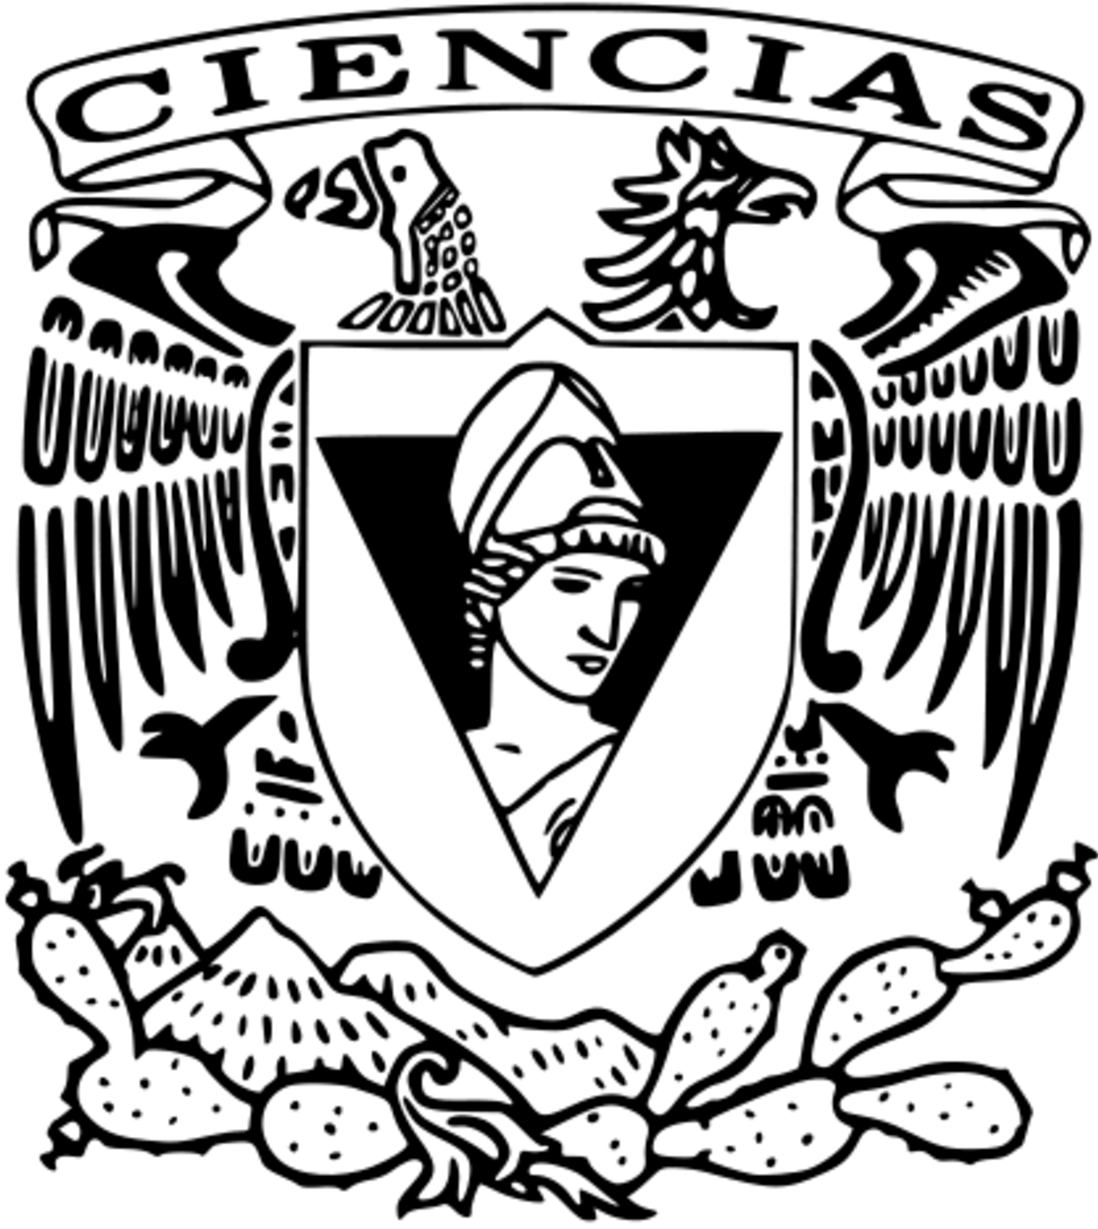
\includegraphics[height=1cm]{Logo_FC.png} \hfill % Inserta un logo a la derecha
  \textit{Página \thepage\ de \pageref{LastPage}}
}

\usetikzlibrary{arrows, backgrounds, shapes.arrows, positioning} % Librerías de TikZ para gráficos vectoriales
\pgfplotsset{compat=newest}   % Asegura la compatibilidad con la versión más reciente de pgfplots

%%%%%%%%%%%%%%%%%%%%%%%%%%%%
% DEFINICIÓN DE ENTORNOS Y COMANDOS
%%%%%%%%%%%%%%%%%%%%%%%%%%%%

% definición del operador para \left( \right)
\newcommand{\paren}[1]{\left({#1}\right)}

% definición del operador para derivada
\newcommand{\dd}[2]{\dfrac{\mathrm{d}#1}{\mathrm{d}#2}}

% definición del operador para la función techo
\newcommand{\techo}[1]{\lceil {#1} \rceil}

% Redefine la numeración de listas para usar números (permite contadores más grandes que el sistema alfabético).
\renewcommand{\theenumi}{\arabic{enumi})}

% Comandos personalizados para mejorar la notación matemática.
\let\emptyset\varnothing         % Utiliza el símbolo \varnothing para el conjunto vacío
\newcommand{\lto}{\mathbin{\to}}   % Define un comando para la flecha "→"

% Redefine los operadores de parte real e imaginaria para evitar conflictos.
\let\Re\relax
\DeclareMathOperator{\Re}{Re}
\let\Im\relax
\DeclareMathOperator{\Im}{Im}

% Definición de entornos para teoremas, corolarios, definiciones y proposiciones.
\newtheorem{teorema}{Teorema}
\newtheorem{corolario}{Corolario}
\newtheorem{definición}{Definición}
\newtheorem{proposición}{Proposición}

%%%%%%%%%%%%%%%%%%%%%%%%%%%%
% INICIO DE DOCUMENTO
%%%%%%%%%%%%%%%%%%%%%%%%%%%%

\begin{document}

%%%%%%%%%%%%%%%%%%%%%%%%%%%%
% ENCABEZADO
%%%%%%%%%%%%%%%%%%%%%%%%%%%%
\begin{center}
    \begin{minipage}{3cm}
    	\begin{center}
    		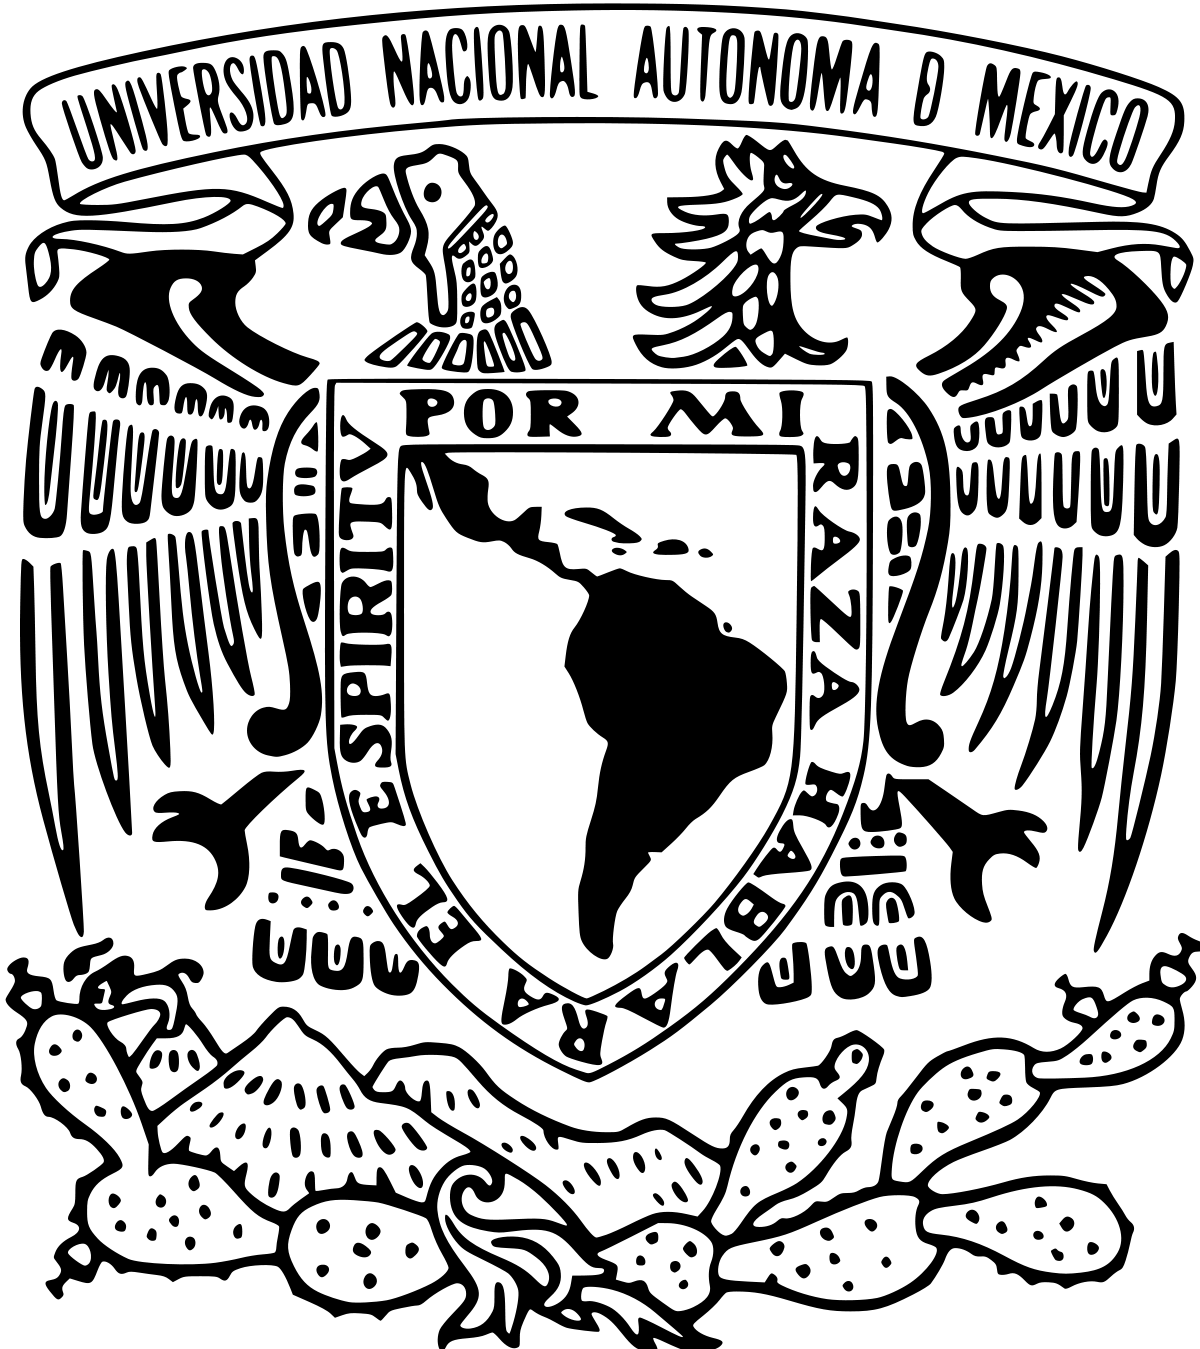
\includegraphics[height=3.4cm]{Logo_UNAM.png}
    	\end{center}
    \end{minipage}\hfill
    \begin{minipage}{10cm}
    	\begin{center}
    	\textbf{\large Universidad Nacional Autónoma de México}\\[0.1cm]
        \textbf{Facultad de Ciencias}\\[0.1cm]
        \textbf{Cálculo Diferencial e Integral IV $|$ Grupo 4176}\\[0.1cm]
        Tarea 1\\[0.1cm]
        Martínez Castro Alvaro Leonardo\\[0.1cm]
        \today
    	\end{center}
    \end{minipage}\hfill
    \begin{minipage}{3cm}
    	\begin{center}
    		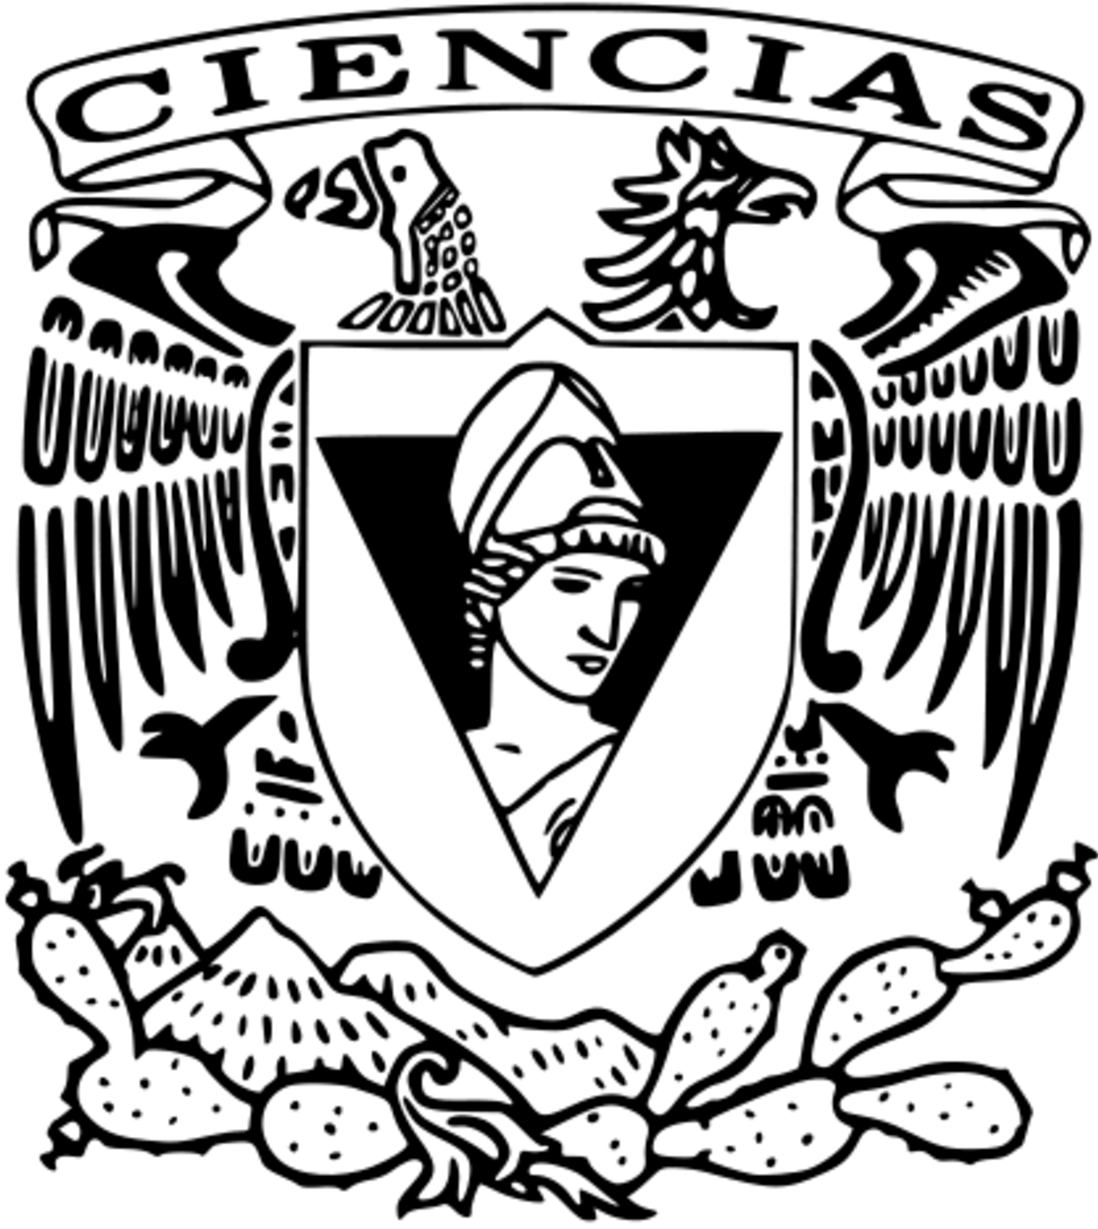
\includegraphics[height=3.4cm]{Logo_FC.png}
    	\end{center}
    \end{minipage}
\end{center}

\rule{17cm}{0.1mm}

%%%%%%%%%%%%%%%%%%%%%%%%%%%%
% FIN DE ENCABEZADO
%%%%%%%%%%%%%%%%%%%%%%%%%%%%


\section*{Rectángulos en $\mathbb{R}^{n}$}

\begin{enumerate}
    \begin{inciso}{Hola}
    \item Sea $R=[a_{1},b_{1}]\times\dots\times[a_{n},b_{n}]$ un rectángulo en $\mathbb{R}^{n}$. Pruebe que:
    \begin{enumerate}
        \item si $b_{i}-a_{i}<\delta$ para $i=1,\dots,n$ entonces $d(R)<\sqrt{n}\cdot\delta$
        \item si $\hat{x},\hat{y}\in R$, entonces $||\hat{x}-\hat{y}||\le d(R)$
        \item si $\hat{x}_{0}\in R$ y $r>d(R)$, entonces $R\subset B_{r}(\hat{x}_{0})$
    \end{enumerate}
    \end{inciso}
    
    \item Pruebe que si $A\subset\mathbb{R}^{n}$ y $R$ es un rectángulo en $\mathbb{R}^{n}$ tal que $R\cap A\neq\emptyset$ y $R\cap A^{c}\neq\emptyset,$ entonces 
    \begin{equation*}
        R\cap \text{Fr}(A)\neq\emptyset
    \end{equation*}
\end{enumerate}

\section*{Particiones e integral}

\begin{enumerate}
    \setcounter{enumi}{2}
    \item Pruebe que, si $f$ es integrable sobre el rectángulo $R\subset\mathbb{R}^{n}$, entonces $f$ es integrable sobre cualquier rectángulo $R^{\prime}\subset R$
    
    \item Sea $f:R\subset\mathbb{R}^{n}\rightarrow\mathbb{R}$ acotada tal que $f(\hat{x})=0$ para toda $\hat{x}\in \text{int}(R).$ Pruebe que $f$ es integrable sobre $R$ y que
    \begin{equation*}
        \int_{R}f=0.
    \end{equation*}
    
    \item Sea $f:R=[0,1]\times[0,1]\rightarrow\mathbb{R}$ definida como:
    \begin{equation*}
        f(x,y)=\begin{cases}
            0 & \text{si } x \text{ o } y \text{ es irracional, } 0 \text{ o } 1\\ 
            \frac{1}{n}+\frac{1}{q} & \text{si } x=\frac{m}{n}, y=\frac{p}{q} \text{ con } (m,n) \text{ y } (p,q) \text{ primos relativos}
        \end{cases}
    \end{equation*}
    Determine si $f$ es integrable sobre $R$. Pruebe su respuesta.
    
    \item Sean $f:R\subset\mathbb{R}^{n}\rightarrow\mathbb{R}$ acotada, $I\in\mathbb{R}$ y $\{\mathcal{P}^{(k)}\}$, $\{Q^{(k)}\}$ dos sucesiones de particiones del rectángulo $R$ tales que
    \begin{equation*}
        \lim_{k\rightarrow\infty}\underline{S}(f,\mathcal{P}^{(k)})=I=\lim_{k\rightarrow\infty}\overline{S}(f,Q^{(k)})
    \end{equation*}
    Pruebe que $f$ es integrable sobre $R$ y que además
    \begin{equation*}
        \int_{R}f=I.
    \end{equation*}
\end{enumerate}

\section*{Propiedades de la integral}

\begin{enumerate}
    \setcounter{enumi}{6}
    \item Sea $f:R\subset\mathbb{R}^{n}\rightarrow\mathbb{R}$ integrable sobre $R$. Pruebe que, si $M$ y $m$ son tales que $m\le f(\hat{x})\le M$ para toda $\hat{x}\in R,$ entonces
    \begin{equation*}
        m\cdot m(R)\le\int_{R}f\le M\cdot m(R).
    \end{equation*}
    
    \item Sean $f,g$ funciones integrables sobre el rectángulo cerrado $R\subset\mathbb{R}^{n}$ y $c\in\mathbb{R}.$ Pruebe que $f+g$ y $cf$ son integrables sobre $R$, y además
    \begin{equation*}
        \int_{R}(f+g)=\int_{R}f+\int_{R}g \quad \text{y} \quad \int_{R}cf=c\int_{R}f.
    \end{equation*}
    
    \item Sean $R$, $R_{1}$, $R_{2}$ rectángulos en $\mathbb{R}^{n}$ tales que $R=R_{1}\cup R_{2}$ e $\text{int}(R_{1})\cap \text{int}(R_{2})=\emptyset$. Pruebe que:
    \begin{enumerate}
        \item 
        \begin{equation*}
            \underline{\int_{R}}f=\underline{\int_{R_{1}}}f+\underline{\int_{R_{2}}}f \quad \text{y} \quad \overline{\int_{R}}f=\overline{\int_{R_{1}}}f+\overline{\int_{R_{2}}}f
        \end{equation*}
        \item $f$ es integrable sobre $R$ si y sólo si $f$ es integrable sobre $R_{1}$ y $R_{2}$. Además, en ambos casos se tiene que:
        \begin{equation*}
            \int_{R}f=\int_{R_{1}}f+\int_{R_{2}}f.
        \end{equation*}
    \end{enumerate}
    
    \item Pruebe que, si $f:R\subset\mathbb{R}^{n}\rightarrow\mathbb{R}$ es integrable sobre $R$, entonces:
    \begin{enumerate}
        \item $f^{+}$ definida como
        \begin{equation*}
            f^{+}(\hat{x})=\begin{cases}
                f(\hat{x}) & \text{si } f(\hat{x})>0,\\ 
                0 & \text{si } f(\hat{x})\le 0,
            \end{cases}
        \end{equation*}
        es integrable sobre $R$.
        \item $f^{-}$ definida como
        \begin{equation*}
            f^{-}(\hat{x})=\begin{cases}
                f(\hat{x}) & \text{si } f(\hat{x})<0,\\ 
                0 & \text{si } f(\hat{x})\ge 0,
            \end{cases}
        \end{equation*}
        es integrable sobre $R$. (Sugerencia: pruebe, y use, que $f=f^{+}+f^{-}$.)
        \item $|f|$ es integrable sobre $R$ y además
        \begin{equation*}
            \left|\int_{R}f\right|\le\int_{R}|f|.
        \end{equation*}
        \item Si además $g:R\subset\mathbb{R}^{n}\rightarrow\mathbb{R}$ es integrable sobre $R$, entonces $\min\{f,g\}$ y $\max\{f,g\}$ son integrables sobre $R$.
    \end{enumerate}
    
    \item Sea $f:R\subset\mathbb{R}^{n}\rightarrow\mathbb{R}$ acotada.
    \begin{enumerate}
        \item Suponga que $f(\hat{x})\ge 0$ para toda $\hat{x}\in R$. Pruebe que, si $M=\sup\{f(\hat{x})\mid\hat{x}\in R\}$, $M^{\prime}=\sup\{f^{2}(\hat{x})\mid\hat{x}\in R\}$, $m=\inf\{f(\hat{x})\mid\hat{x}\in R\}$ y $m^{\prime}=\inf\{f^{2}(\hat{x})\mid\hat{x}\in R\}$, entonces $M^{\prime}=M^{2}$ y $m^{\prime}=m^{2}.$ ¿Es indispensable la hipótesis de que $f$ sea no negativa? Justifique su respuesta.
        \item Pruebe que, si $f$ es integrable sobre $R$ entonces $f^{2}$ es integrable sobre $R$.
        \item Pruebe que, si $f$ y $g$ son integrables sobre $R$ entonces $fg$ es integrable sobre $R$.
    \end{enumerate}
    
    \item Sea $f:R\subset\mathbb{R}^{n}\rightarrow\mathbb{R}$ acotada. Pruebe que, si $f^{2}$ es integrable sobre $R$ entonces $|f|$ es integrable sobre $R$. ¿$f$ es integrable sobre $R$?
    
    \item Sea $f:R\subset\mathbb{R}^{n}\rightarrow\mathbb{R}$ integrable sobre $R$ tal que $f(\hat{x})\le 0$ para toda $\hat{x}\in R$. Pruebe que:
    \begin{enumerate}
        \item 
        \begin{equation*}
            \int_{R}f\le 0
        \end{equation*}
        \item Si $f$ es continua en $\hat{x}_{0}\in R$ y $f(\hat{x}_{0})<0$, entonces
        \begin{equation*}
            \int_{R}f<0
        \end{equation*}
        \item Si $f$ es menor que cero para toda $\hat{x}\in R$ entonces
        \begin{equation*}
            \int_{R}f<0
        \end{equation*}
    \end{enumerate}
\end{enumerate}

\section*{Conjuntos Jordan medibles}

\begin{enumerate}
    \setcounter{enumi}{13}
    \item Sean $A, B\subset\mathbb{R}^{n}$ acotados. Pruebe que:
    \begin{enumerate}
        \item si $J(B)=J(A)=0$ entonces $J(A\cup B)=0$
        \item si $B\subset A$ y $J(A)=0$ entonces $B$ es Jordan-medible y además $J(B)=0$
    \end{enumerate}
    
    \item Sea $A\subset\mathbb{R}^{n}$ un conjunto Jordan-medible. Pruebe que:
    \begin{enumerate}
        \item $J(A)>0\Leftrightarrow \text{int}(A)\neq\emptyset$
        \item $J(A)=0\Leftrightarrow A\subset \text{Fr}(A)$
        \item $\text{int}(A)$ es Jordan-medible y además $J(\text{int}(A))=J(A)$
        \item si $B$ es un conjunto tal que $\text{int}(A)\subseteq B\subseteq(A\cup \text{Fr}(A))$, entonces $B$ es Jordan-medible y además
        \begin{equation*}
            J(B)=J(A)
        \end{equation*}
    \end{enumerate}
    
    \item Sea $\{A_{k}\subset\mathbb{R}^{n}\mid k\in\mathbb{N}\}$ una familia de conjuntos Jordan-medibles tales que $\bigcup_{k=1}^{\infty}A_{k}$ y $\bigcap_{k=1}^{\infty}A_{k}$ son acotados. ¿Los conjuntos $\bigcup_{k=1}^{\infty}A_{k}$ y $\bigcap_{k=1}^{\infty}A_{k}$ son Jordan-medibles? Pruebe su respuesta.
    
    \item Sean $A, B\subset\mathbb{R}^{n}$ Jordan-medibles. Pruebe que $A\setminus B$ es Jordan-medible y además
    \begin{equation*}
        J(A\setminus B)=J(A)-J(A\cap B)
    \end{equation*}
    
    \item Sea $f:R\subset\mathbb{R}^{n}\rightarrow\mathbb{R}$ integrable sobre el rectángulo $R$ tal que $D_{f,R}$ es un conjunto Jordan-medible. Pruebe que $J(D_{f,R})=0$.
\end{enumerate}

\section*{Integral sobre conjuntos Jordan medibles}

\begin{enumerate}
    \setcounter{enumi}{18}
    \item Sea $f:A\subset\mathbb{R}^{n}\rightarrow\mathbb{R}$, tal que $J(A)=0$ y $f$ es acotada sobre $A$. Pruebe que $f$ es integrable sobre $A$ y además
    \begin{equation*}
        \int_{A}f=0.
    \end{equation*}
    
    \item Sea $f:A\subset\mathbb{R}^{n}\rightarrow\mathbb{R}$ acotada sobre el conjunto Jordan-medible $A$. Pruebe que, si $f(\hat{x})=0$ para toda $\hat{x}\in \text{int}(A)$ entonces $f$ es integrable sobre $A$ y además
    \begin{equation*}
        \int_{A}f=0.
    \end{equation*}
    
    \item Sea $f:A\subset\mathbb{R}^{n}\rightarrow\mathbb{R}$ acotada sobre el conjunto Jordan-medible $A$ y $R$ un rectángulo tal que $A\subset R$. Pruebe que
    \begin{equation*}
        D_{f_{A},R}\subset \text{Fr}(A)\cup D_{f,A}
    \end{equation*}
    ¿Es necesaria la hipótesis de que $A$ sea un conjunto Jordan-medible? Pruebe su respuesta.
    
    \item Sea $f:A\subset\mathbb{R}^{n}\rightarrow\mathbb{R}$ integrable sobre el conjunto Jordan-medible $A$. Pruebe que la gráfica de $f$
    \begin{equation*}
        G_{f}=\{(\hat{x},f(\hat{x}))\in\mathbb{R}^{n+1}\mid\hat{x}\in A\}
    \end{equation*}
    es un conjunto Jordan-medible en $\mathbb{R}^{n+1}$ y de medida de Jordan cero.
    
    \item Sean $f,g:A\subset\mathbb{R}^{n}\rightarrow\mathbb{R}$ continuas sobre el conjunto cerrado, acotado y Jordan-medible $A$, tales que $f(\hat{x})\le g(\hat{x})$ para toda $\hat{x}\in A$. Pruebe que el conjunto
    \begin{equation*}
        \{(\hat{x},y)\in\mathbb{R}^{n+1}\mid f(\hat{x})\le y\le g(\hat{x}),\hat{x}\in A\}
    \end{equation*}
    es Jordan-medible en $\mathbb{R}^{n+1}$.
    
    \item Sea $f:A\subset\mathbb{R}^{n}\rightarrow\mathbb{R}$ integrable sobre $A$ y $B\subset A$.
    \begin{enumerate}
        \item ¿$f$ es integrable sobre $B$? Pruebe su respuesta.
        \item ¿Bajo qué condiciones sobre $B$ es cierto que $f$ es integrable sobre $B$? Pruebe su respuesta.
        \item Pruebe que, si $f$ es integrable sobre $B$, entonces $f$ es integrable sobre $A\setminus B$.
        \item Pruebe que, si $f$ es integrable sobre $B$ y además $f(\hat{x})\ge 0$ para toda $\hat{x}\in A,$ entonces
        \begin{equation*}
            \int_{B}f\le\int_{A}f.
        \end{equation*}
    \end{enumerate}
    
    \item Sean $A, B, C\subset\mathbb{R}^{n}$ tales que $A=B\cup C$. Pruebe que, si $f:A\subset\mathbb{R}^{n}\rightarrow\mathbb{R}$ es integrable sobre $A$, sobre $A\setminus B$ y sobre $A\setminus C$ entonces $f$ es integrable sobre $B,$ sobre $C$ y sobre $B\cap C,$ y además
    \begin{equation*}
        \int_{A}f=\int_{B}f+\int_{C}f-\int_{B\cap C}f.
    \end{equation*}
    
    \item Sea $f:A\subset\mathbb{R}^{n}\rightarrow\mathbb{R}$ integrable sobre el conjunto Jordan-medible $A$ tal que $f(\hat{x})\ge 0$ para toda $\hat{x}\in A$. Pruebe que, si $f$ es continua en $\hat{x}_{0}\in \text{int}(A)$ y $f(\hat{x}_{0})>0$, entonces
    \begin{equation*}
        \int_{A}f>0.
    \end{equation*}
    ¿Es indispensable la hipótesis de que $\hat{x}_{0}\in \text{int}(A)$?
    
    \item Sea $f:A\subset\mathbb{R}^{n}\rightarrow\mathbb{R}$ integrable sobre el conjunto Jordan-medible $A$. Suponga que $f(\hat{x})\ge 0$ para toda $\hat{x}\in A$ y sea $B=\{\hat{x}\in A\mid f(\hat{x})>0\}$. Pruebe que
    \begin{equation*}
        \int_{A}f>0
    \end{equation*}
    si y sólo si $\text{int}(B)\neq\emptyset$.
    
    \item Sea $f:A\subset\mathbb{R}^{n}\rightarrow\mathbb{R}$ integrable sobre el conjunto Jordan-medible $A$. Sea $B=\{\hat{x}\in A\mid f(\hat{x})\neq 0\}.$
    \begin{enumerate}
        \item ¿$B$ es un conjunto Jordan-medible?
        \item Pruebe que $f$ es integrable sobre $B$ y que además
        \begin{equation*}
            \int_{A}f=\int_{B}f.
        \end{equation*}
    \end{enumerate}
\end{enumerate}


\end{document}


